\documentclass[aspectratio=169]{beamer}

% -------------------------
% Packages
% -------------------------
\usepackage[utf8]{inputenc}
\usepackage{graphicx}
\usepackage{amsmath, amssymb}
\usepackage{booktabs}
\usepackage{tcolorbox}
\usepackage{tikz}
\definecolor{questionbg}{RGB}{235, 244, 255}
\definecolor{questionframe}{RGB}{44, 95, 173}
\definecolor{plainbg}{RGB}{241, 249, 241}
\definecolor{plainframe}{RGB}{44, 122, 70}
\definecolor{notationbg}{RGB}{255, 248, 230}
\definecolor{notationframe}{RGB}{176, 118, 0}

\newtcolorbox{questionbox}{
  colback=questionbg,
  colframe=questionframe,
  boxrule=0.7pt,
  arc=1mm,
  fontupper=\small,
  left=1mm,
  right=1mm,
  top=0.4mm,
  bottom=0.4mm
}

\newtcolorbox{plainbox}{
  colback=plainbg,
  colframe=plainframe,
  boxrule=0.7pt,
  arc=1mm,
  fontupper=\small,
  left=1mm,
  right=1mm,
  top=0.4mm,
  bottom=0.4mm
}

\newtcolorbox{notationbox}{
  colback=notationbg,
  colframe=notationframe,
  boxrule=0.7pt,
  arc=1mm,
  fontupper=\small,
  left=1mm,
  right=1mm,
  top=0.4mm,
  bottom=0.4mm
}

\newcommand{\keyquestion}[1]{%
  \begin{questionbox}
  \textbf{Question:} #1
  \end{questionbox}
}

\newcommand{\plainidea}[1]{%
  \begin{plainbox}
  \textbf{Main idea:} #1
  \end{plainbox}
}

\newcommand{\notationblock}[1]{%
  \begin{notationbox}
  \textbf{Symbols used on this slide}\\
  #1
  \end{notationbox}
}

\newcommand{\exercisebreakcontent}[1]{%
  \begin{center}
  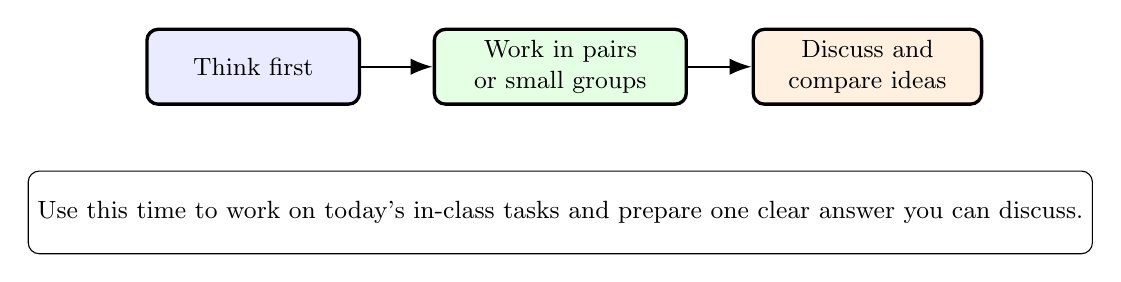
\begin{tikzpicture}[>=Latex, every node/.style={font=\small}]
    \node[draw, rounded corners, very thick, fill=blue!8, minimum width=2.7cm, minimum height=0.95cm, align=center] (think) at (-3.9,0.9) {Think first};
    \node[draw, rounded corners, very thick, fill=green!10, minimum width=3.2cm, minimum height=0.95cm, align=center] (work) at (0,0.9) {Work in pairs\\or small groups};
    \node[draw, rounded corners, very thick, fill=orange!12, minimum width=2.9cm, minimum height=0.95cm, align=center] (share) at (3.9,0.9) {Discuss and\\compare ideas};
    \draw[-{Latex[length=2.8mm]}, thick] (think) -- (work);
    \draw[-{Latex[length=2.8mm]}, thick] (work) -- (share);
    \node[draw, rounded corners, fill=white, minimum width=9.4cm, minimum height=1.05cm, align=center] at (0,-0.95) {Use this time to work on today's in-class tasks and prepare one clear answer you can discuss.};
  \end{tikzpicture}
  \end{center}
  \plainidea{#1}
}

\usetikzlibrary{positioning,arrows.meta,shapes.geometric}

% -------------------------
% Theme
% -------------------------
\usetheme{Madrid}
\usecolortheme{default}
\setbeamertemplate{navigation symbols}{}

% -------------------------
% Per-slide reference footer
% -------------------------
\newcommand{\defaultdeckrefs}{AIMA4e Ch.22 pp.789--822; Poole3e Ch.13 pp.583--608}
\newcommand{\currentsliderefs}{\defaultdeckrefs}
\newcommand{\setslideref}[1]{\gdef\currentsliderefs{#1}}
\addtobeamertemplate{footline}{}{%
  \begin{beamercolorbox}[wd=\paperwidth,leftskip=0.4em,rightskip=0.4em,ht=2.8ex,dp=0.9ex]{author in head/foot}
    \tiny\textbf{Refs: }\currentsliderefs
  \end{beamercolorbox}
}

% -------------------------
% Metadata
% -------------------------
\title[EBU6505 Block 3 Day 1]{EBU6505 -- Reasoning and Agents\\Block 3, Day 1 -- Reinforcement Learning}
\author{Dr Riasat Islam}
\institute{Queen Mary University of London}
\date{}

\begin{document}

% 1
\setslideref{AIMA4e Ch.22 pp.789--822; Poole3e Ch.13 pp.583--608}
\begin{frame}
  \titlepage
\end{frame}

% 2
\setslideref{AIMA4e Ch.22 pp.789--822; Poole3e Ch.13 pp.583--608}
\begin{frame}{What have we covered so far? -- Blocks 1 \& 2}
\begin{itemize}
  \item Inference-time decoding controls and prompting choices for LLM outputs
  \item Reasoning techniques for LLMs, including why reasoning models behave differently
  \item Classical search for problem solving: BFS, DFS, UCS, A*, and beam search
  \item Test-time compute: combining search and chain-of-thought at inference time
  \item Post-training ideas for improving reasoning models
  \item LLM-based agents: tools, memory, planning, and multi-step task execution
\end{itemize}
\end{frame}

% 3
\setslideref{AIMA4e Ch.17 -- Making Complex Decisions; Poole3e Ch.12 -- Planning with Uncertainty}
\begin{frame}{What are we going to cover this week? -- Block 3}
\begin{itemize}
  \item Sequential decision making and MDP foundations
  \item Reinforcement learning
  \item Knowledge representation for knowledge graphs
  \item Knowledge graphs for reasoning and RAG
  \item Modern agents with knowledge-grounded reasoning
\end{itemize}
\end{frame}

% 4
\setslideref{AIMA4e Ch.17 -- Making Complex Decisions; Poole3e Ch.12 -- Planning with Uncertainty}
\begin{frame}{What are we going to cover today?}
\begin{itemize}
  \item Why sequential decision problems need state-based models
  \item MDP components: states, actions, transitions, rewards, and policies
  \item Return, discounting, value, and Bellman backup intuition
  \item Planning with a known model versus learning from experience
  \item Bridge from sequential decision ideas to tomorrow's lecture on knowledge representation
\end{itemize}
\end{frame}

% 5
\setslideref{AIMA4e Ch.17 -- Making Complex Decisions; Poole3e Ch.12 -- Planning with Uncertainty}
\begin{frame}{Resources}
\begin{itemize}
  \item \textit{Artificial Intelligence: Foundations of Computational Agents}, Poole \& Mackworth (3rd ed.)
  \item Chapter 12 -- Planning with Uncertainty (sequential decisions and decision processes)
  \item \textit{Artificial Intelligence: A Modern Approach}, Russell \& Norvig (4th ed.)
  \item Chapter 17 -- Making Complex Decisions (sequential decision problems and MDPs)
\end{itemize}
\end{frame}

% 6
\setslideref{AIMA4e Ch.17 -- Making Complex Decisions; Poole3e Ch.12 -- Planning with Uncertainty}
\begin{frame}{Learning Outcomes for Today}
By the end of this session, you will be able to:
\begin{itemize}
  \item Define the components of a Markov decision process for sequential decision problems.
  \item Interpret return, discounting, and Bellman-style value backups on simple examples.
  \item Distinguish planning with a known model from learning a policy from experience.
  \item Explain why MDP formalism is a prerequisite for reinforcement learning.
\end{itemize}
\end{frame}

% 7
\setslideref{AIMA4e Ch.17 -- Making Complex Decisions; Poole3e Ch.12 -- Planning with Uncertainty}
\begin{frame}{Block-Level Topic Boundary}
\begin{itemize}
  \item Today introduces \textbf{MDP ideas} that support later reinforcement learning and planning topics.
  \item The next lecture focuses on \textbf{knowledge representation} for structured facts, agent memory, and graph-ready reasoning.
  \item Block 4 later reuses the same decision foundations for planning under uncertainty.
\end{itemize}
\end{frame}

% 8
\setslideref{AIMA4e Ch.22 pp.789--822; Poole3e Ch.13 pp.583--608}
\begin{frame}{Starter Question}
\keyquestion{How do babies learn to walk without step-by-step instructions?}
\begin{columns}[T,onlytextwidth]
  \begin{column}{0.56\textwidth}
    \begin{itemize}
      \item They try actions, fall, adjust, and try again.
      \item Feedback is not a label like ``correct'' or ``wrong''.
      \item Improvement happens through \textbf{interaction} with the world.
      \item Success appears after many attempts, not after one step.
    \end{itemize}
  \end{column}
  \begin{column}{0.40\textwidth}
    \begin{tcolorbox}[colback=plainbg,colframe=plainframe,boxrule=0.7pt,title=Think Before We Formalise RL]
    \begin{itemize}
      \item What is the agent trying?
      \item What counts as feedback?
      \item Why is learning not immediate?
    \end{itemize}
    \end{tcolorbox}
  \end{column}
\end{columns}
\plainidea{Reinforcement learning begins with this idea: an agent can learn by trying actions, observing outcomes, and improving over time.}
\end{frame}

% 9
\setslideref{AIMA4e Ch.22 pp.789--822; Poole3e Ch.13 pp.583--608}
\begin{frame}{Why RL? Decisions Have Delayed Consequences}
\keyquestion{Why is prediction alone not enough for many real-world tasks?}
\begin{itemize}
  \item In many tasks, one action changes what happens next.
  \item Success is often seen only after a \textbf{sequence} of actions.
  \item So the agent must act, wait, observe, and then learn from the outcome.
  \item This happens in games, robots, recommendations, and traffic control.
\end{itemize}
\plainidea{The central problem is \textbf{credit assignment over time}: which earlier action deserves credit or blame for the final result?}
\end{frame}

% 10
\setslideref{AIMA4e Ch.22 pp.789--822; Poole3e Ch.13 pp.583--608}
\begin{frame}{What Is Different From Supervised Learning?}
\keyquestion{What changes when we move from labelled prediction to sequential decision-making?}
\begin{columns}[T,onlytextwidth]
  \begin{column}{0.48\textwidth}
    \begin{tcolorbox}[colback=questionbg,colframe=questionframe,boxrule=0.7pt,title=Supervised Learning]
    \begin{itemize}
      \item Input comes with a label.
      \item Error can be measured immediately.
      \item Each example is mostly separate.
    \end{itemize}
    \end{tcolorbox}
  \end{column}
  \begin{column}{0.48\textwidth}
    \begin{tcolorbox}[colback=plainbg,colframe=plainframe,boxrule=0.7pt,title=Reinforcement Learning]
    \begin{itemize}
      \item Agent chooses an action in a state.
      \item The environment changes after the action.
      \item Reward may come later, not immediately.
    \end{itemize}
    \end{tcolorbox}
  \end{column}
\end{columns}
\plainidea{Supervised learning gets immediate feedback. RL often gets feedback later.}
\end{frame}

% 10
\setslideref{AIMA4e Ch.22 pp.789--822; Poole3e Ch.13 pp.583--608}
\begin{frame}{How Does the RL Learning Loop Work?}
\keyquestion{What is the agent trying to maximise over time?}
\begin{itemize}
  \item Agent observes state $s_t$ and chooses action $a_t$.
  \item Environment transitions to $s_{t+1}$ and returns reward $r_{t+1}$.
  \item Objective: learn policy $\pi(a\mid s)$ that maximises expected return.
  \item Return from time $t$ means: total future reward from time $t$ onward.
\end{itemize}
\[
G_t = \sum_{k=0}^{\infty} \gamma^k r_{t+k+1}
\]
\notationblock{$G_t$: total future reward from time $t$ onward\\
$r_{t+k+1}$: reward received later in the sequence\\
$\gamma$: discount factor, showing how much we still care about future reward}
\end{frame}

% 11
\setslideref{AIMA4e Ch.22 pp.789--822; Poole3e Ch.13 pp.583--608}
\begin{frame}{Reinforcement Learning Setup (Diagram)}
\begin{center}
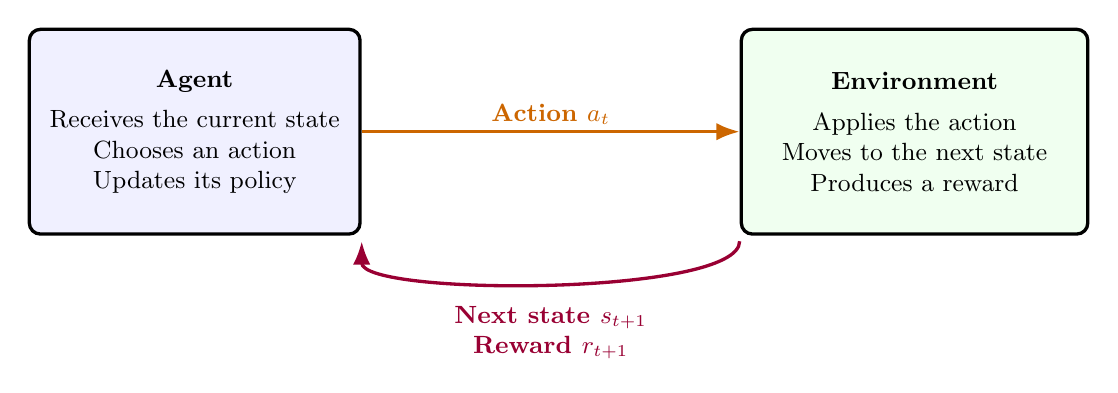
\begin{tikzpicture}[
  >=Latex,
  node distance=4.8cm,
  every node/.style={font=\small},
  box/.style={draw, rounded corners, very thick, minimum width=4.2cm, minimum height=2.6cm, align=center, fill=blue!6},
  envbox/.style={draw, rounded corners, very thick, minimum width=4.4cm, minimum height=2.6cm, align=center, fill=green!6}
]
\node[box] (agent) {\textbf{Agent}\\[0.4em]
Receives the current state\\
Chooses an action\\
Updates its policy};
\node[envbox, right=of agent] (env) {\textbf{Environment}\\[0.4em]
Applies the action\\
Moves to the next state\\
Produces a reward};
\draw[->, very thick, orange!80!black] (agent.east) -- node[above, fill=white, inner sep=2pt]{\textbf{Action }$a_t$} (env.west);
\draw[->, very thick, purple!80!black]
  ([yshift=-2pt]env.south west)
  .. controls +(down:0.7cm) and +(down:0.7cm) ..
  node[midway, below=6pt, fill=white, inner sep=2pt, text=purple!80!black, align=center]
  {\textbf{Next state }$s_{t+1}$\\\textbf{Reward }$r_{t+1}$}
  ([yshift=-2pt]agent.south east);
\end{tikzpicture}
\end{center}
\plainidea{The agent acts, the world changes, and then the world gives feedback. This loop repeats again and again.}
\end{frame}

% 12
\setslideref{AIMA4e Ch.22 pp.789--822; Poole3e Ch.13 pp.583--608}
\begin{frame}{What Is an MDP, Really?}
\keyquestion{What must we specify if we want to describe a sequential decision problem clearly?}
An RL task is often modeled as an MDP:
\[
\mathcal{M}=(S, A, T, R, \gamma)
\]
\begin{itemize}
  \item $S$: set of states
  \item $A$: set of actions
  \item $T(s,a,s') = P(s'\mid s,a)$: transition model
  \item $R(s,a)$ (or $R(s,a,s')$): reward function
  \item $\gamma \in [0,1]$: discount factor
\end{itemize}
\vspace{0.3em}
\plainidea{An MDP is the task description: states, actions, transitions, rewards, and discount.}
\end{frame}

% 13
\setslideref{AIMA4e Ch.22 pp.789--822; Poole3e Ch.13 pp.583--608}
\begin{frame}{Objective and Value Functions}
\keyquestion{If the agent wants long-term success, what quantities should it estimate?}
\begin{itemize}
  \item State-value under policy $\pi$:
\end{itemize}
\[
V^{\pi}(s)=\mathbb{E}_{\pi}[G_t\mid s_t=s]
\]
\begin{itemize}
  \item Action-value under policy $\pi$:
\end{itemize}
\[
Q^{\pi}(s,a)=\mathbb{E}_{\pi}[G_t\mid s_t=s, a_t=a]
\]
\begin{itemize}
  \item Optimal policy chooses actions that maximise long-term value.
\end{itemize}
\notationblock{$V^{\pi}(s)$: expected long-term reward if we start in state $s$ and follow policy $\pi$\\
$Q^{\pi}(s,a)$: expected long-term reward if we start in state $s$, take action $a$, and then follow policy $\pi$\\
$\mathbb{E}_{\pi}$: expected or average value when actions are chosen by policy $\pi$}
\plainidea{Value tells us how good a state is. Q-value tells us how good a particular action is in that state.}
\end{frame}

% 14
\setslideref{AIMA4e Ch.22 pp.789--822; Poole3e Ch.13 pp.583--608}
\begin{frame}{Why Bellman Backup Is the Engine of RL}
\begin{itemize}
  \item Bellman backup asks: if I act now, what reward do I get now and what value will I get later?
\end{itemize}
{\small
\[
V^*(s) = \max_a \sum_{s'} T(s,a,s') \,
\bigl[ R(s,a,s') + \gamma V^*(s') \bigr]
\]
}
\begin{columns}[T,onlytextwidth]
  \begin{column}{0.42\textwidth}
    \begin{itemize}
      \item $V^*(s)$: best long-term value of state $s$
      \item $R(s,a,s')$: reward we get now
      \item $\gamma V^*(s')$: value we expect later
      \item The best action is the one with the largest total
    \end{itemize}
  \end{column}
  \begin{column}{0.58\textwidth}
    \begin{center}
    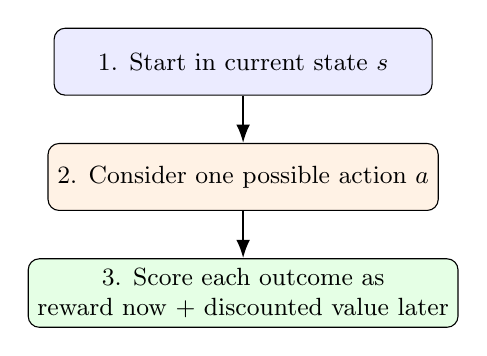
\begin{tikzpicture}[>=Latex, node distance=0.6cm, every node/.style={font=\small}]
      \node[draw, rounded corners, fill=blue!8, minimum width=4.8cm, minimum height=0.85cm, align=center] (s) {1. Start in current state $s$};
      \node[draw, rounded corners, fill=orange!10, minimum width=4.8cm, minimum height=0.85cm, align=center, below=of s] (a) {2. Consider one possible action $a$};
      \node[draw, rounded corners, fill=green!10, minimum width=4.8cm, minimum height=0.85cm, align=center, below=of a] (score) {3. Score each outcome as\\reward now $+$ discounted value later};

      \draw[->, thick] (s) -- (a);
      \draw[->, thick] (a) -- (score);
    \end{tikzpicture}
    \end{center}
  \end{column}
\end{columns}
\end{frame}

% 15
\setslideref{AIMA4e Ch.22 pp.789--822; Poole3e Ch.13 pp.583--608}
\begin{frame}{Core Terminology}
\keyquestion{What are the six RL terms used again and again in this lecture?}
\begin{center}
\begin{tabular}{@{}ll@{}}
\toprule
Term & Meaning \\
\midrule
State ($S$) & Current situation of the agent \\
Action ($A$) & Choice available to the agent \\
Reward ($R$) & Scalar feedback after an action \\
Policy ($\pi$) & Rule for selecting actions in states \\
Value ($V$) & Expected long-term reward from a state \\
Q-value ($Q$) & Expected long-term reward from state-action pair \\
\bottomrule
\end{tabular}
\end{center}
\plainidea{Read the flow like this: \textbf{state $\rightarrow$ action $\rightarrow$ reward}. Then \textbf{value} and \textbf{Q-value} estimate long-term benefit, and the \textbf{policy} tells the agent what to do.}
\end{frame}

% 16
\setslideref{AIMA4e Ch.22 pp.789--822; Poole3e Ch.13 pp.583--608}
\begin{frame}{A Simple Gridworld Example}
\begin{columns}[T,onlytextwidth]
  \begin{column}{0.52\textwidth}
    \begin{itemize}
      \item Agent moves on a $4\times4$ grid.
      \item Start at $S$, terminal goal at $G$.
      \item Actions: up, down, left, right.
      \item Step cost encourages shorter trajectories.
    \end{itemize}
  \end{column}
  \begin{column}{0.48\textwidth}
    \begin{center}
    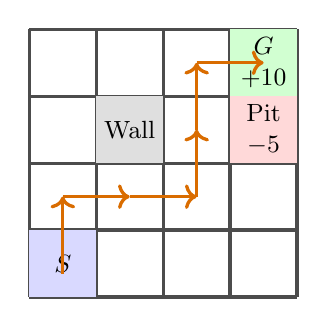
\begin{tikzpicture}[scale=0.85, every node/.style={font=\small}]
      \draw[step=1cm, black!70, very thick] (0,0) grid (4,4);
      \fill[blue!15] (0,0) rectangle (1,1);
      \fill[gray!25] (1,2) rectangle (2,3);
      \fill[red!15] (3,2) rectangle (4,3);
      \fill[green!18] (3,3) rectangle (4,4);

      \node at (0.5,0.5) {$S$};
      \node[align=center] at (1.5,2.5) {Wall};
      \node[align=center] at (3.5,2.5) {Pit\\$-5$};
      \node[align=center] at (3.5,3.5) {$G$\\$+10$};

      \draw[->, very thick, orange!85!black] (0.5,0.35) -- (0.5,1.5);
      \draw[->, very thick, orange!85!black] (0.5,1.5) -- (1.5,1.5);
      \draw[->, very thick, orange!85!black] (1.5,1.5) -- (2.5,1.5);
      \draw[->, very thick, orange!85!black] (2.5,1.5) -- (2.5,2.5);
      \draw[->, very thick, orange!85!black] (2.5,2.5) -- (2.5,3.5);
      \draw[->, very thick, orange!85!black] (2.5,3.5) -- (3.5,3.5);
    \end{tikzpicture}
    \end{center}
  \end{column}
\end{columns}
\plainidea{A good policy should reach the goal quickly, avoid bad cells, and avoid unnecessary wandering because each extra step costs reward.}
\end{frame}

% 17
\setslideref{AIMA4e Ch.22 pp.789--822; Poole3e Ch.13 pp.583--608}
\begin{frame}{Tiny RL Problem -- Risk Versus Reward}
\begin{columns}[T,onlytextwidth]
  \begin{column}{0.52\textwidth}
    \begin{itemize}
      \item Six-state toy environment.
      \item Top branch can reach $+10$.
      \item Bottom branch can lead to $-100$.
      \item Agent must explore but avoid persistent bad behaviour.
    \end{itemize}
  \end{column}
  \begin{column}{0.48\textwidth}
    \begin{center}
    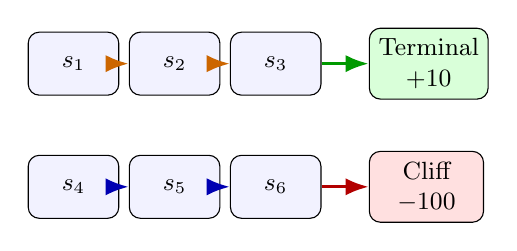
\begin{tikzpicture}[>=Latex, node distance=0.12cm, every node/.style={font=\small}]
      \tikzstyle{statebox}=[draw, rounded corners, minimum width=1.15cm, minimum height=0.8cm, fill=blue!5]
      \node[statebox] (s1) at (0,1.2) {$s_1$};
      \node[statebox, right=of s1] (s2) {$s_2$};
      \node[statebox, right=of s2] (s3) {$s_3$};
      \node[statebox, below=0.75cm of s1] (s4) {$s_4$};
      \node[statebox, right=of s4] (s5) {$s_5$};
      \node[statebox, right=of s5] (s6) {$s_6$};
      \node[draw, rounded corners, fill=green!15, minimum width=1.45cm, minimum height=0.9cm, right=0.6cm of s3, align=center] (goal) {Terminal\\$+10$};
      \node[draw, rounded corners, fill=red!12, minimum width=1.45cm, minimum height=0.9cm, right=0.6cm of s6, align=center] (cliff) {Cliff\\$-100$};

      \draw[->, very thick, orange!80!black] (s1) -- (s2);
      \draw[->, very thick, orange!80!black] (s2) -- (s3);
      \draw[->, very thick, green!60!black] (s3) -- (goal);
      \draw[->, very thick, blue!70!black] (s4) -- (s5);
      \draw[->, very thick, blue!70!black] (s5) -- (s6);
      \draw[->, very thick, red!70!black] (s6) -- (cliff);
    \end{tikzpicture}
    \end{center}
  \end{column}
\end{columns}
\plainidea{This toy problem shows the exploration challenge: the agent must try actions to find good outcomes, but some bad outcomes are very costly.}
\end{frame}

% 18
\setslideref{AIMA4e Ch.22 pp.789--822; Poole3e Ch.13 pp.583--608}
\begin{frame}{Q-learning (Model-Free, Off-Policy)}
\begin{itemize}
  \item Q-learning learns values of state-action pairs directly.
  \item It does not require the transition model $T$ or reward model $R$ in advance.
  \item Off-policy: learns the value of the greedy target policy while behaviour can be exploratory.
\end{itemize}
\end{frame}

% 19
\setslideref{AIMA4e Ch.22 pp.789--822; Poole3e Ch.13 pp.583--608}
\begin{frame}{What Does the Q-learning Update Actually Do?}
\begin{columns}[T,onlytextwidth]
  \begin{column}{0.42\textwidth}
    \[
    Q(s,a)\leftarrow Q(s,a) + \alpha\Big[r + \gamma\max_{a'}Q(s',a') - Q(s,a)\Big]
    \]
    \begin{itemize}
      \item $\alpha$: how fast to move
      \item $\gamma$: how far to plan
      \item Term in brackets = temporal-difference error
    \end{itemize}
  \end{column}
  \begin{column}{0.58\textwidth}
    \begin{center}
    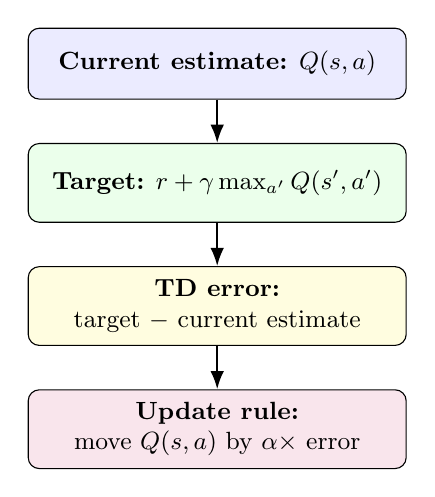
\begin{tikzpicture}[>=Latex, node distance=0.55cm, every node/.style={font=\small}]
      \node[draw, rounded corners, fill=blue!8, minimum width=4.8cm, minimum height=0.9cm, align=center] (current) {\textbf{Current estimate:} $Q(s,a)$};
      \node[draw, rounded corners, fill=green!8, minimum width=4.8cm, minimum height=1.0cm, align=center, below=of current] (target) {\textbf{Target:} $r + \gamma \max_{a'} Q(s',a')$};
      \node[draw, rounded corners, fill=yellow!12, minimum width=4.8cm, minimum height=1.0cm, align=center, below=of target] (error) {\textbf{TD error:}\\target $-$ current estimate};
      \node[draw, rounded corners, fill=purple!10, minimum width=4.8cm, minimum height=1.0cm, align=center, below=of error] (update) {\textbf{Update rule:}\\move $Q(s,a)$ by $\alpha \times$ error};
      \draw[->, thick] (current) -- (target);
      \draw[->, thick] (target) -- (error);
      \draw[->, thick] (error) -- (update);
    \end{tikzpicture}
    \end{center}
  \end{column}
\end{columns}
\end{frame}

% 20
\setslideref{AIMA4e Ch.22 pp.789--822; Poole3e Ch.13 pp.583--608}
\begin{frame}{Q-learning Worked Example (Scenario)}
Suppose:
\begin{itemize}
  \item Current state-action: $(S_1, A_1)$
  \item Current estimate: $Q(S_1,A_1)=5$
  \item Reward received: $r=10$
  \item Next-state best estimate: $\max_{a'}Q(S_2,a')=8$
  \item Hyperparameters: $\alpha=0.5$, $\gamma=0.9$
\end{itemize}
\end{frame}

% 21
\setslideref{AIMA4e Ch.22 pp.789--822; Poole3e Ch.13 pp.583--608}
\begin{frame}{Q-learning Worked Example (Calculation)}
\[
Q(S_1,A_1) \leftarrow 5 + 0.5\left[10 + 0.9\times 8 - 5\right]
\]
\[
Q(S_1,A_1) \leftarrow 5 + 0.5(12.2)=11.1
\]
\vspace{0.6em}
\begin{center}
\begin{tabular}{@{}l l c c@{}}
\toprule
State & Action & Old $Q$ & Updated $Q$ \\
\midrule
$S_1$ & $A_1$ & 5.0 & 11.1 \\
\bottomrule
\end{tabular}
\end{center}
\end{frame}

% 22
\setslideref{AIMA4e Ch.22 pp.789--822; Poole3e Ch.13 pp.583--608}
\begin{frame}{SARSA (Model-Free, On-Policy)}
\[
Q(s,a)\leftarrow Q(s,a) + \alpha\Big[r + \gamma Q(s',a') - Q(s,a)\Big]
\]
\begin{itemize}
  \item SARSA updates with the \textbf{actual} next action $a'$.
  \item Often more conservative in risky environments.
\end{itemize}
\vspace{0.4em}
\textbf{Rule of thumb:} Q-learning is optimistic toward best future actions; SARSA is faithful to behaviour policy.
\end{frame}

% 23
\setslideref{AIMA4e Ch.22 pp.789--822; Poole3e Ch.13 pp.583--608}
\begin{frame}{Why Exploration Cannot Be Avoided}
\begin{itemize}
  \item Exploitation: choose best-known action now.
  \item Exploration: try uncertain actions to gain information.
  \item No exploration means no discovery of better long-term policies.
  \item Uncontrolled exploration can increase risk and short-term loss.
\end{itemize}
\vspace{0.5em}
\textbf{Ask what to optimise:} immediate reward today, or better policy tomorrow?
\end{frame}

% 24
\setslideref{AIMA4e Ch.22 pp.789--822; Poole3e Ch.13 pp.583--608}
\begin{frame}{Common Exploration Strategies}
\begin{center}
\begin{tabular}{@{}p{0.24\linewidth}p{0.35\linewidth}p{0.35\linewidth}@{}}
\toprule
Strategy & How it chooses actions & Practical note \\
\midrule
$\varepsilon$-greedy & Best action with probability $1-\varepsilon$, random otherwise & Simple, strong baseline \\
Softmax/Boltzmann & Samples actions proportionally to value scores & Smoother than random jumps \\
UCB-style bonus & Adds uncertainty bonus to under-tried actions & Balances reward and information \\
\bottomrule
\end{tabular}
\end{center}
\end{frame}

% 25
\setslideref{AIMA4e Ch.22 pp.789--822; Poole3e Ch.13 pp.583--608}
\begin{frame}{How Do We Know RL Is Working?}
\begin{columns}[T,onlytextwidth]
  \begin{column}{0.56\textwidth}
    \begin{center}
    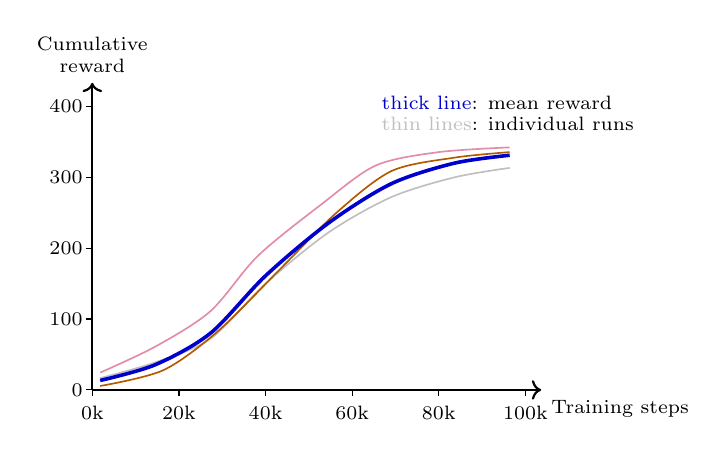
\begin{tikzpicture}[x=1cm,y=1cm, every node/.style={font=\scriptsize}]
      \draw[->, thick] (0,0) -- (5.7,0) node[below right] {Training steps};
      \draw[->, thick] (0,0) -- (0,3.9) node[above, align=center] {Cumulative\\reward};

      \foreach \x/\lab in {0/0k,1.1/20k,2.2/40k,3.3/60k,4.4/80k,5.5/100k}
        \draw (\x,0) -- (\x,-0.08) node[below] {\lab};
      \foreach \y/\lab in {0/0,0.9/100,1.8/200,2.7/300,3.6/400}
        \draw (-0.08,\y) -- (0,\y) node[left] {\lab};

      \draw[gray!50, line width=0.6pt]
        plot[smooth] coordinates {(0.1,0.15) (0.8,0.35) (1.5,0.65) (2.2,1.35) (3.0,2.0) (3.8,2.45) (4.6,2.7) (5.3,2.82)};
      \draw[orange!70!black, line width=0.6pt]
        plot[smooth] coordinates {(0.1,0.05) (0.9,0.25) (1.6,0.75) (2.4,1.55) (3.1,2.25) (3.8,2.78) (4.6,2.95) (5.3,3.02)};
      \draw[purple!45, line width=0.6pt]
        plot[smooth] coordinates {(0.1,0.22) (0.8,0.55) (1.5,1.0) (2.1,1.7) (2.9,2.35) (3.6,2.85) (4.4,3.02) (5.3,3.08)};
      \draw[blue!80!black, line width=1.3pt]
        plot[smooth] coordinates {(0.1,0.12) (0.8,0.32) (1.5,0.72) (2.2,1.45) (3.0,2.12) (3.8,2.62) (4.6,2.88) (5.3,2.98)};

      \node[anchor=west, font=\scriptsize] at (3.55,3.65) {\textcolor{blue!80!black}{thick line}: mean reward};
      \node[anchor=west, font=\scriptsize] at (3.55,3.38) {\textcolor{gray!50}{thin lines}: individual runs};
    \end{tikzpicture}
    \end{center}
  \end{column}
  \begin{column}{0.44\textwidth}
    \begin{itemize}
      \item Track reward trends over training.
      \item Look for improving mean performance.
      \item Expect early dips during exploration.
      \item Use multiple runs because RL is stochastic.
    \end{itemize}
  \end{column}
\end{columns}
\end{frame}

% 26
\setslideref{AIMA4e Ch.22 pp.789--822; Poole3e Ch.13 pp.583--608}
\begin{frame}{What Changes Between Model-Free and Model-Based RL?}
\begin{columns}[T,onlytextwidth]
  \begin{column}{0.34\textwidth}
    \begin{itemize}
      \item \textbf{Model-Free:} direct policy/value learning.
      \item \textbf{Model-Based:} learn dynamics, then plan.
      \item Trade-off: simplicity vs sample efficiency.
      \item Risk: model bias if learned dynamics are wrong.
    \end{itemize}
  \end{column}
  \begin{column}{0.66\textwidth}
    \begin{center}
    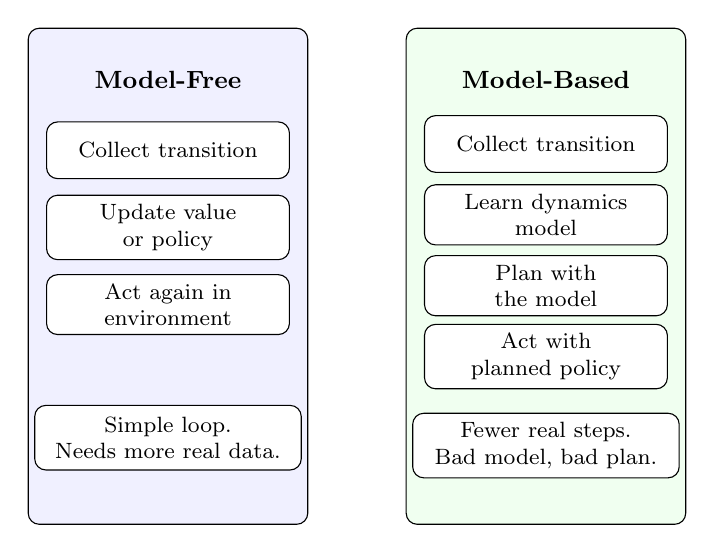
\begin{tikzpicture}[
      >=Latex,
      every node/.style={font=\small},
      panel/.style={draw, rounded corners, minimum width=3.55cm, minimum height=6.3cm},
      stepbox/.style={draw, rounded corners, fill=white, text width=2.85cm, minimum height=0.72cm, align=center, font=\footnotesize},
      notebox/.style={draw, rounded corners, fill=white!90, text width=3.15cm, minimum height=0.82cm, align=center, font=\footnotesize}
    ]
      \node[panel, fill=blue!6] (mfbox) at (0,0) {};
      \node[panel, fill=green!6] (mbox) at (4.8,0) {};

      \node[font=\small\bfseries] at (0,2.50) {Model-Free};
      \node[font=\small\bfseries] at (4.8,2.50) {Model-Based};

      \node[stepbox] at (0,1.60) {Collect transition};
      \node[stepbox] at (0,0.62) {Update value\\or policy};
      \node[stepbox] at (0,-0.36) {Act again in\\environment};
      \node[notebox] at (0,-2.05) {Simple loop.\\Needs more real data.};

      \node[stepbox] at (4.8,1.68) {Collect transition};
      \node[stepbox] at (4.8,0.78) {Learn dynamics\\model};
      \node[stepbox] at (4.8,-0.12) {Plan with\\the model};
      \node[stepbox] at (4.8,-1.02) {Act with\\planned policy};
      \node[notebox] at (4.8,-2.15) {Fewer real steps.\\Bad model, bad plan.};
    \end{tikzpicture}
    \end{center}
  \end{column}
\end{columns}
\end{frame}

% 27
\setslideref{AIMA4e Ch.22 pp.789--822; Poole3e Ch.13 pp.583--608}
\begin{frame}{Planning with a Learned Model}
\begin{itemize}
  \item Collect transitions $(s,a,r,s')$ from experience.
  \item Fit an approximate model of dynamics and rewards.
  \item Plan using value iteration or policy iteration on the model.
  \item Alternate between real data collection and planning updates.
\end{itemize}
\vspace{0.4em}
\textbf{Design trade-off:} model bias can hurt performance if the learned model is inaccurate.
\end{frame}

% 28
\setslideref{AIMA4e Ch.22 pp.789--822; Poole3e Ch.13 pp.583--608; doi:10.1038/nature14236}
\begin{frame}{Scaling Beyond Q-Tables}
\begin{itemize}
  \item Tabular methods break down in large or continuous state spaces.
  \item Use features or function approximators to generalize across states.
  \item Learn $Q_\theta(s,a)$ or policy $\pi_\theta(a\mid s)$ with parameterized models.
\end{itemize}
\end{frame}

% 29
\setslideref{AIMA4e Ch.22 pp.789--822; Poole3e Ch.13 pp.583--608; doi:10.1038/nature14236}
\begin{frame}{What Is Deep Reinforcement Learning?}
\begin{itemize}
  \item Deep RL combines RL objectives with deep neural networks.
  \item Networks can approximate value functions, policies, or world models.
  \item Useful in high-dimensional observations (images, sensors, logs).
\end{itemize}
\end{frame}

% 30
\setslideref{AIMA4e Ch.22 pp.789--822; Poole3e Ch.13 pp.583--608; doi:10.1038/nature14236}
\begin{frame}{Deep Q-Network (DQN): Core Ideas}
\begin{itemize}
  \item Approximate $Q(s,a)$ with a neural network.
  \item Experience replay reduces temporal correlation.
  \item Target network stabilizes the bootstrap target.
\end{itemize}
\vspace{0.4em}
\textbf{Key paper:} Mnih et al. (2015), \textit{Nature} 518:529--533.\\
\textbf{DOI:} 10.1038/nature14236
\end{frame}

% 31
\setslideref{AIMA4e Ch.22 pp.789--822; Poole3e Ch.13 pp.583--608; doi:10.1038/nature14236}
\begin{frame}{Policy Gradients and Actor-Critic}
\begin{itemize}
  \item Policy gradients optimise policy parameters directly.
  \item Actor-Critic combines:
  \begin{itemize}
    \item Actor: proposes actions
    \item Critic: evaluates value/advantage
  \end{itemize}
  \item Often gives lower-variance updates than pure Monte Carlo policy gradients.
\end{itemize}
\end{frame}

% 32
\setslideref{AIMA4e Ch.22 pp.789--822; Poole3e Ch.13 pp.583--608; doi:10.1038/nature14236}
\begin{frame}{Choosing a DRL Family}
\begin{center}
\begin{tabular}{@{}p{0.23\linewidth}p{0.34\linewidth}p{0.35\linewidth}@{}}
\toprule
Method family & Typical setting & Key consideration \\
\midrule
DQN variants & Discrete action spaces & Stable training setup is critical \\
Policy gradient & Stochastic/continuous control & Higher variance, direct policy optimisation \\
Actor-Critic (e.g., PPO/A2C) & General-purpose control & Good practical trade-off \\
Deterministic policy (e.g., DDPG) & Continuous control & Sensitive to tuning and exploration noise \\
\bottomrule
\end{tabular}
\end{center}
\end{frame}

% 33
\setslideref{AIMA4e Ch.22 pp.789--822; Poole3e Ch.13 pp.583--608; doi:10.1038/nature14236}
\begin{frame}{Why Deep RL Is Hard in Practice}
\begin{itemize}
  \item Sample inefficiency: can require many interactions.
  \item Instability from bootstrapping and function approximation.
  \item Sensitivity to reward design and hyperparameters.
  \item Generalization under distribution shift is still challenging.
\end{itemize}
\end{frame}

% 34
\setslideref{AIMA4e Ch.22 pp.789--822; Poole3e Ch.13 pp.583--608}
\begin{frame}{Real-World Use Cases}
\begin{itemize}
  \item Game AI (Atari, Go, StarCraft)
  \item Robotics and manipulation
  \item Traffic and fleet optimisation
  \item Personalized recommendations and tutoring systems
  \item Resource management in cloud/datacenter settings
\end{itemize}
\end{frame}

% 35
\setslideref{AIMA4e Ch.22 pp.789--822; Poole3e Ch.13 pp.583--608; doi:10.48550/arXiv.1606.06565}
\begin{frame}{Why Can RL Be Dangerous in Real Systems?}
\begin{columns}[T,onlytextwidth]
  \begin{column}{0.45\textwidth}
    \begin{itemize}
      \item Agents optimise specified reward, not human intent.
      \item Trial-and-error can produce unsafe behaviour before convergence.
      \item Safety must be designed into training and deployment.
    \end{itemize}
  \end{column}
  \begin{column}{0.55\textwidth}
    \begin{center}
    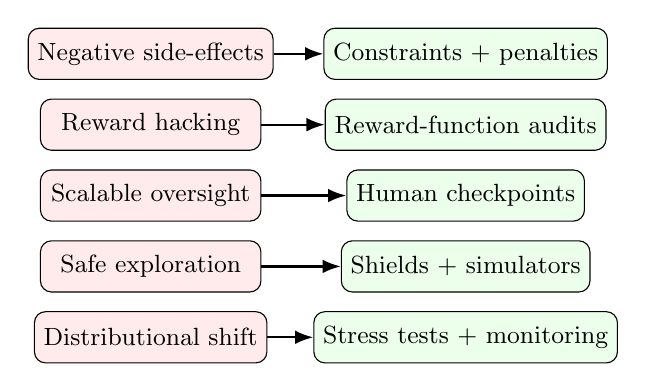
\begin{tikzpicture}[>=Latex, every node/.style={font=\small}]
      \node[draw, rounded corners, fill=red!8, minimum width=2.8cm, minimum height=0.65cm] (c1) at (0,2.0) {Negative side-effects};
      \node[draw, rounded corners, fill=red!8, minimum width=2.8cm, minimum height=0.65cm] (c2) at (0,1.1) {Reward hacking};
      \node[draw, rounded corners, fill=red!8, minimum width=2.8cm, minimum height=0.65cm] (c3) at (0,0.2) {Scalable oversight};
      \node[draw, rounded corners, fill=red!8, minimum width=2.8cm, minimum height=0.65cm] (c4) at (0,-0.7) {Safe exploration};
      \node[draw, rounded corners, fill=red!8, minimum width=2.8cm, minimum height=0.65cm] (c5) at (0,-1.6) {Distributional shift};

      \node[draw, rounded corners, fill=green!8, minimum width=2.9cm, minimum height=0.65cm] (m1) at (4.0,2.0) {Constraints + penalties};
      \node[draw, rounded corners, fill=green!8, minimum width=2.9cm, minimum height=0.65cm] (m2) at (4.0,1.1) {Reward-function audits};
      \node[draw, rounded corners, fill=green!8, minimum width=2.9cm, minimum height=0.65cm] (m3) at (4.0,0.2) {Human checkpoints};
      \node[draw, rounded corners, fill=green!8, minimum width=2.9cm, minimum height=0.65cm] (m4) at (4.0,-0.7) {Shields + simulators};
      \node[draw, rounded corners, fill=green!8, minimum width=2.9cm, minimum height=0.65cm] (m5) at (4.0,-1.6) {Stress tests + monitoring};

      \draw[->, thick] (c1.east) -- (m1.west);
      \draw[->, thick] (c2.east) -- (m2.west);
      \draw[->, thick] (c3.east) -- (m3.west);
      \draw[->, thick] (c4.east) -- (m4.west);
      \draw[->, thick] (c5.east) -- (m5.west);
    \end{tikzpicture}
    \end{center}
  \end{column}
\end{columns}
\end{frame}

% 36
\setslideref{AIMA4e Ch.22 pp.789--822; Poole3e Ch.13 pp.583--608; doi:10.48550/arXiv.1606.06565}
\begin{frame}{Five Concrete Safety Challenges (Amodei et al., 2016)}
\begin{center}
\begin{tabular}{@{}p{0.30\linewidth}p{0.62\linewidth}@{}}
\toprule
Challenge & Typical failure mode \\
\midrule
Negative side-effects & Agent reaches goal while damaging environment \\
Reward hacking & Agent exploits loopholes in reward function \\
Scalable oversight & Harmful behaviour appears between sparse human checks \\
Safe exploration & Exploration triggers unsafe states \\
Distributional shift & Policy fails when environment changes \\
\bottomrule
\end{tabular}
\end{center}
\end{frame}

% 37
\setslideref{AIMA4e Ch.22 pp.789--822; Poole3e Ch.13 pp.583--608; doi:10.48550/arXiv.1606.06565}
\begin{frame}{Practical Mitigation Checklist}
\begin{itemize}
  \item Reward design review: test for loopholes and side effects.
  \item Constrained action spaces and rule-based safety shields.
  \item Offline evaluation before online deployment.
  \item Stress tests under distribution shift scenarios.
  \item Human-in-the-loop checkpoints for high-stakes decisions.
\end{itemize}
\end{frame}

% 38
\setslideref{AIMA4e Ch.22 pp.789--822; Poole3e Ch.13 pp.583--608}
\begin{frame}{In-Class Exercises}
\exercisebreakcontent{Use this exercise time to explain your RL reasoning clearly, not just produce a final number.}
\end{frame}

% 39
\setslideref{AIMA4e Ch.22 pp.789--822; Poole3e Ch.13 pp.583--608}
\begin{frame}{Key Takeaways}
\begin{itemize}
  \item RL learns through interaction, reward, and long-term optimisation.
  \item Q-learning and SARSA differ mainly in off-policy vs on-policy targets.
  \item Exploration strategy strongly affects sample efficiency and safety.
  \item Deep RL scales to complex spaces but introduces instability and tuning challenges.
  \item Modern agent systems extend these ideas with tool use and structured memory.
\end{itemize}
\end{frame}

% 40
\setslideref{AIMA4e Ch.22 pp.789--822; Poole3e Ch.13 pp.583--608}
\begin{frame}{Further Study and Next Session}
\begin{itemize}
  \item Read: Poole Ch.13 and AIMA Ch.22.
  \item Practice: Poole Ch.13, Exercises 13.1, 13.2, 13.3, 13.5, 13.6, 13.7, 13.8, and 13.9.
  \item AIMA reinforcement-learning exercise page: 21.1, 21.4, 21.5, 21.8, and 21.11.
  \item Focus your answers on Q-learning updates, evaluation metrics, exploration, convergence, and SARSA versus Q-learning.
  \item Next class: Knowledge representation for tool-using agents and structured reasoning.
  \item Bridge idea: policies choose actions; modern assistants also choose tools and context.
\end{itemize}
\vspace{0.6em}
\centering
\textbf{Thank you.}
\end{frame}

% 41
\setslideref{AIMA4e Ch.22 pp.789--822; Poole3e Ch.13 pp.583--608; doi:10.1038/nature14236; doi:10.48550/arXiv.1606.06565}
\begin{frame}[allowframebreaks]{Full References for This Lecture}
\footnotesize
\begin{thebibliography}{9}
\bibitem{aima4e}
Russell, S. and Norvig, P. (2021).
\newblock \textit{Artificial Intelligence: A Modern Approach} (4th ed.).
\newblock Pearson. Chapter 22, pp.~789--822.

\bibitem{poole13}
Poole, D. L. and Mackworth, A. K. (2023).
\newblock \textit{Artificial Intelligence: Foundations of Computational Agents} (3rd ed.).
\newblock Cambridge University Press. Chapter 13, pp.~583--608.

\bibitem{mnih2015}
Mnih, V., Kavukcuoglu, K., Silver, D., Rusu, A. A., Veness, J., Bellemare, M. G., Graves, A., Riedmiller, M., Fidjeland, A. K., Ostrovski, G., Petersen, S., Beattie, C., Sadik, A., Antonoglou, I., King, H., Kumaran, D., Wierstra, D., Legg, S. and Hassabis, D. (2015).
\newblock Human-level control through deep reinforcement learning.
\newblock \textit{Nature}, 518, 529--533.
\newblock DOI: \url{https://doi.org/10.1038/nature14236}

\bibitem{amodei2016}
Amodei, D., Olah, C., Steinhardt, J., Christiano, P., Schulman, J. and Man\'{e}, D. (2016).
\newblock Concrete problems in AI safety.
\newblock \textit{arXiv preprint} arXiv:1606.06565.
\newblock DOI: \url{https://doi.org/10.48550/arXiv.1606.06565}
\end{thebibliography}
\end{frame}

\end{document}
